\documentclass[a4paper,12pt,oneside]{article}
\usepackage{graphicx}
\usepackage{hyperref}
\usepackage[T1]{fontenc}
\usepackage[utf8]{inputenc}
\usepackage{setspace}
\usepackage{amsmath}
\usepackage{amssymb}

\begin{document}

    \thispagestyle{plain}
    \begin{center}
        \normalsize
        \textbf{Assignment 1}
            
        \vspace{0.2cm}
        \normalsize
        21/10/2022
            
        \vspace{0.2cm}
        \textbf{Francesco Refolli 865955}
    \end{center}

    \paragraph{Il Problema}
    
    \begin{align*}
        Max \; Z &= x_1 - 2 x_2 \\
        x_1 - x_2 & \geq 1 \\
        x_1 - 2 x_2 & \leq 6 \\
        2 x_1 - x_2 & \leq 6 \\
        x_1 & \geq 0 \\
        x_2 & \leq 0
    \end{align*}

    \section{Risolvere il problema primale con l’algoritmo del simplesso}

    \paragraph{Conversione del problema in forma aumentata}
    Per poter risolvere il problema primale usando l'algoritmo del simplesso devo convertire prima il problema in forma aumentata. \\
    Voglio tutti i vincoli di segno al $\geq$, quindi creo la variabile $y = - x_2$, pongo il vincolo $y \geq 0$ e sostituisco $y = -x_2$ in tutti i vincoli e nella funzione obiettivo.

    \begin{align*}
        Max \; Z &= x_1 + 2 y \\
        x_1 + y & \geq 1 \\
        x_1 + 2 y & \leq 6 \\
        2 x_1 + y & \leq 6 \\
        x_1, y & \geq 0
    \end{align*}

    Quindi aggiungo una variabile surplus al vincolo 1: $x_3$.

    \begin{align*}
        Max \; Z &= x_1 + 2 y \\
        x_1 + y - x_3 & = 1 \\
        x_1 + 2 y & \leq 6 \\
        2 x_1 + y & \leq 6 \\
        x_1, y & \geq 0
    \end{align*}

    Quindi aggiungo due variabile slack ai vincolo 2 e 3: $x_4, x_5$.

    \begin{align*}
        Max \; Z &= x_1 + 2 y \\
        x_1 + y - x_3 & = 1 \\
        x_1 + 2 y + x_4 & = 6 \\
        2 x_1 + y + x_5 & = 6 \\
        x_1, y & \geq 0
    \end{align*}

    \paragraph{Forma tabellare}

    \begin{center}
        \begin{tabular}{||c c c c c c c c||}
            \hline
            base & Z & $x_1$ & $y$ & $x_3$ & $x_4$ & $x_5$ & b \\
            \hline
            \hline
            & 1 & -1 & -2 &  0 & 0 & 0 & 0 \\
            \hline
            & 0 &  1 &  1 & -1 & 0 & 0 & 1 \\
            \hline
            & 0 &  1 &  2 &  0 & 1 & 0 & 6 \\
            \hline
            & 0 &  2 &  1 &  0 & 0 & 1 & 6 \\
            \hline
        \end{tabular}
    \end{center}

    La soluzione di partenza (0, 0, -1, 6, 6) non e' ammissibile quindi introduco una variabile artificiale $A \geq 0$.

    \begin{center}
        \begin{tabular}{||c c c c c c c c c||}
            \hline
            base & Z & $x_1$ & $y$ & $x_3$ & $x_4$ & $x_5$ & A & b \\
            \hline
            \hline
            Z     & 1 & -1 & -1 &  1 & 0 & 0 & 0 & -1 \\
            \hline
            A     & 0 &  1 &  1 & -1 & 0 & 0 & 1 &  1 \\
            \hline
            $x_4$ & 0 &  1 &  2 &  0 & 1 & 0 & 0 &  6 \\
            \hline
            $x_5$ & 0 &  2 &  1 &  0 & 0 & 1 & 0 &  6 \\
            \hline
        \end{tabular}
    \end{center}

    In questo modo ottengo la soluzione di base ammissibile (0,0,0,1,6,6).

    \paragraph{Iterazione 0}

    $x_1$ e $y$ hanno entrambe coefficiente -1 in prima riga, quindi scelgo arbitrariamente $x_1$.
    Calcolando i rapporti dei coefficienti in colonna strettamente positivi, la riga 1 con rapporto $\frac 1 1 = 1$, ha rapporto minimo.
    Quindi la variabile di base uscente e' $A$, la variabile non di base entrante e' $x_1$.
    Ricalcolo le righe di conseguenza. Il risultato dell'iterazione e':

    \begin{center}
        \begin{tabular}{||c c c c c c c c c||}
            \hline
            base & Z & $x_1$ & $y$ & $x_3$ & $x_4$ & $x_5$ & A & b \\
            \hline
            \hline
            Z     & 1 &  0 &  0 &  0 & 0 & 0 &  1 &  0 \\
            \hline
            $x_1$ & 0 &  1 &  1 & -1 & 0 & 0 &  1 &  1 \\
            \hline
            $x_4$ & 0 &  0 &  1 &  1 & 1 & 0 & -1 &  5 \\
            \hline
            $x_5$ & 0 &  0 & -1 &  2 & 0 & 1 & -2 &  4 \\
            \hline
        \end{tabular}
    \end{center}

    La variabile A e' uscita dalla base, non ci sono piu' variabili artificiali nella base, quindi trasformo il tableau per risolvere il problema originale.
    Sostituisco la riga 0 con la funzione obiettivo originale. Quindi annullo i coefficienti in riga 0 corrispondenti alle variabili in base sottraendo una combinazione lineare delle righe 1,2,3.
    Ottengo:

    \begin{center}
        \begin{tabular}{||c c c c c c c c||}
            \hline
            base & Z & $x_1$ & $y$ & $x_3$ & $x_4$ & $x_5$ & b \\
            \hline
            \hline
            Z     & 1 &  0 & -1 & -1 & 0 & 0 &  1 \\
            \hline
            $x_1$ & 0 &  1 &  1 & -1 & 0 & 0 &  1 \\
            \hline
            $x_4$ & 0 &  0 &  1 &  1 & 1 & 0 &  5 \\
            \hline
            $x_5$ & 0 &  0 & -1 &  2 & 0 & 1 &  4 \\
            \hline
        \end{tabular}
    \end{center}

    \paragraph{Iterazione 1}

    $x_3$ e $y$ hanno entrambe coefficiente -1 in prima riga, quindi scelgo arbitrariamente $y$.
    Calcolando i rapporti dei coefficienti in colonna strettamente positivi, la riga 1 con rapporto $\frac 1 1 = 1$, ha rapporto minimo.
    Quindi la variabile di base uscente e' $x_1$, la variabile non di base entrante e' $y$.
    Ricalcolo le righe di conseguenza. Il risultato dell'iterazione e':

    \begin{center}
        \begin{tabular}{||c c c c c c c c||}
            \hline
            base & Z & $x_1$ & $y$ & $x_3$ & $x_4$ & $x_5$ & b \\
            \hline
            \hline
            Z     & 1 &  1 &  0 & -2 & 0 & 0 &  2 \\
            \hline
            $y$   & 0 &  1 &  1 & -1 & 0 & 0 &  1 \\
            \hline
            $x_4$ & 0 & -1 &  0 &  2 & 1 & 0 &  4 \\
            \hline
            $x_5$ & 0 &  1 &  0 &  1 & 0 & 1 &  5 \\
            \hline
        \end{tabular}
    \end{center}

    \paragraph{Iterazione 2}
    
    $x_3$ ha coefficiente -2 in prima riga, quindi lo scelgo come variabile entrante.
    Calcolando i rapporti dei coefficienti in colonna strettamente positivi, la riga 2 con rapporto $\frac 4 2 = 2$, ha rapporto minimo.
    Quindi la variabile di base uscente e' $x_4$, la variabile non di base entrante e' $x_3$.
    Ricalcolo le righe di conseguenza. Il risultato dell'iterazione e':

    \begin{center}
        \begin{tabular}{||c c c c c c c c||}
            \hline
            base & Z & $x_1$ & $y$ & $x_3$ & $x_4$ & $x_5$ & b \\
            \hline
            \hline
            Z     & 1 &            0 &  0 &  0 &            1 & 0 &  6 \\
            \hline
            $y$   & 0 &  $\frac 1 2$ &  1 &  0 &  $\frac 1 2$ & 0 &  3 \\
            \hline
            $x_3$ & 0 & -$\frac 1 2$ &  0 &  1 &  $\frac 1 2$ & 0 &  2 \\
            \hline
            $x_5$ & 0 &  $\frac 3 2$ &  0 &  0 & -$\frac 1 2$ & 1 &  3 \\
            \hline
        \end{tabular}
    \end{center}

    \paragraph{iterazione 3}
    
    La prima riga non contiene piu' valori negativi, l'algoritmo del simplesso si arresta. \\
    La soluzione di base corrente e' ($x_1$,$y$,$x_3$,$x_4$,$x_5$) = (0,3,2,0,3) \\
    Quindi una soluzione al problema PL e' ($x_1$,$y$) = (0,3). \\
    Tuttavia ricordando $y = -x_2$, e' piu' significativo dire ($x_1$, $x_2$) = (0, -3).
    
    Ad ogni modo, siccome una delle variabili non di base ha coefficiente 0 in prima posizione e' possibile continuare con le iterazioni per individuare una ulteriore soluzione ottimale al problema PL. \\

    Seleziono quindi $x_1$ che ha coefficiente 0.
    Calcolando i rapporti dei coefficienti in colonna strettamente positivi, la riga 3 con rapporto $\frac 3 {\frac 3 2} = 2$, ha rapporto minimo.
    Quindi la variabile di base uscente e' $x_5$, la variabile non di base entrante e' $x_1$.
    Ricalcolo le righe di conseguenza. Il risultato dell'iterazione e':

    \begin{center}
        \begin{tabular}{||c c c c c c c c||}
            \hline
            base & Z & $x_1$ & $y$ & $x_3$ & $x_4$ & $x_5$ & b \\
            \hline
            \hline
            Z     & 1 & 0 & 0 & 0 &            1 &            0 &  6 \\
            \hline
            $y$   & 0 & 0 & 1 & 0 &  $\frac 2 3$ & -$\frac 1 3$ &  2 \\
            \hline
            $x_3$ & 0 & 0 & 0 & 1 &  $\frac 1 3$ &  $\frac 1 3$ &  3 \\
            \hline
            $x_1$ & 0 & 1 & 0 & 0 & -$\frac 1 3$ &  $\frac 2 3$ &  2 \\
            \hline
        \end{tabular}
    \end{center}

    \paragraph{iterazione 4}

    La prima riga non contiene valori negativi, l'algoritmo del simplesso si arresta. \\
    La soluzione di base corrente e' ($x_1$,$y$,$x_3$,$x_4$,$x_5$) = (2,2,3,0,0) \\
    Quindi un'altra soluzione al problema PL e' ($x_1$,$y$) = (2,2)\\
    Tuttavia ricordando $y = -x_2$, e' piu' significativo dire ($x_1$, $x_2$) = (2, -2). \\

    Essendoci due soluzioni ottimali di base, tutte le soluzioni ottimali sono una combinazione convessa delle due precedentemente ottenute: \\
    ($x_1, x_2, x_3, x_4, x_5$) = $w_1 \cdot $ (0,-3,2,0,3) $+$ $w_2 \cdot $ (2,-2,3,0,0)

    \newpage

    \section{Risolverlo il problema primale graficamente}

    Costruisco il grafico con le equazioni dei vincoli lungo l'asse $x_1 \times x_2$.

    \begin{center}
        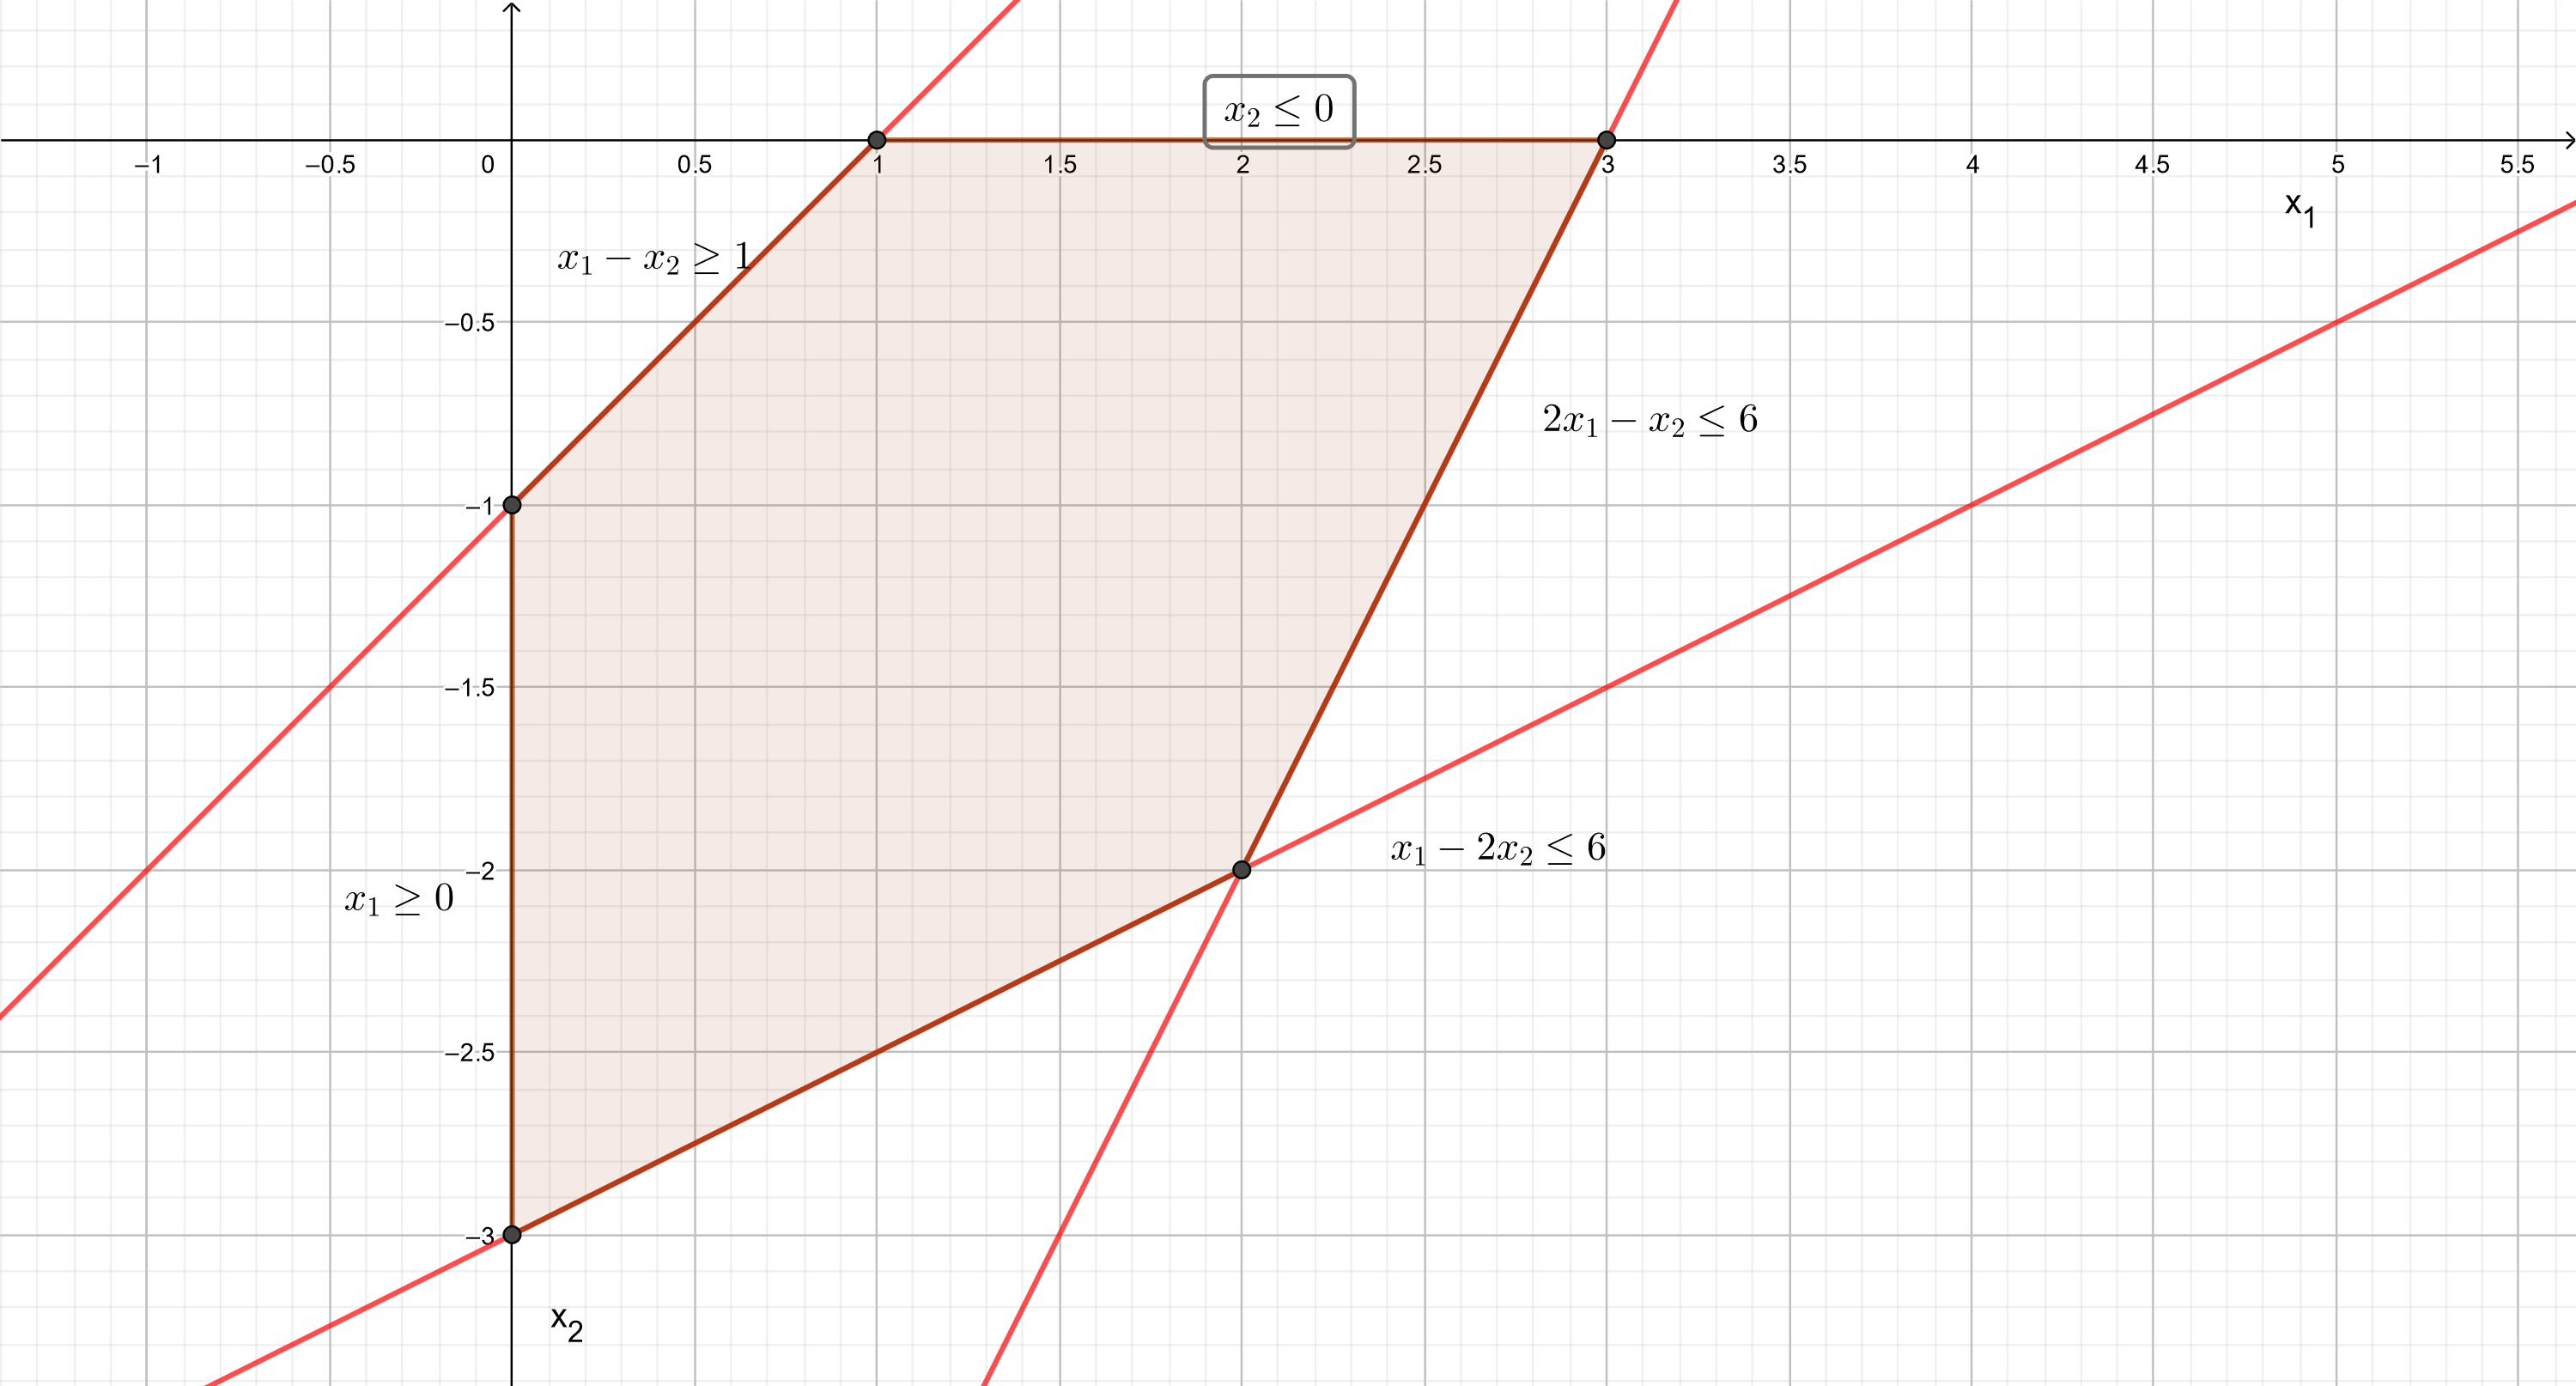
\includegraphics[width=12cm]{prima-fase.png}
    \end{center}

    Quindi disegno il gradiente della funzione obiettivo $g$ e la funzione obiettivo.

    \begin{center}
        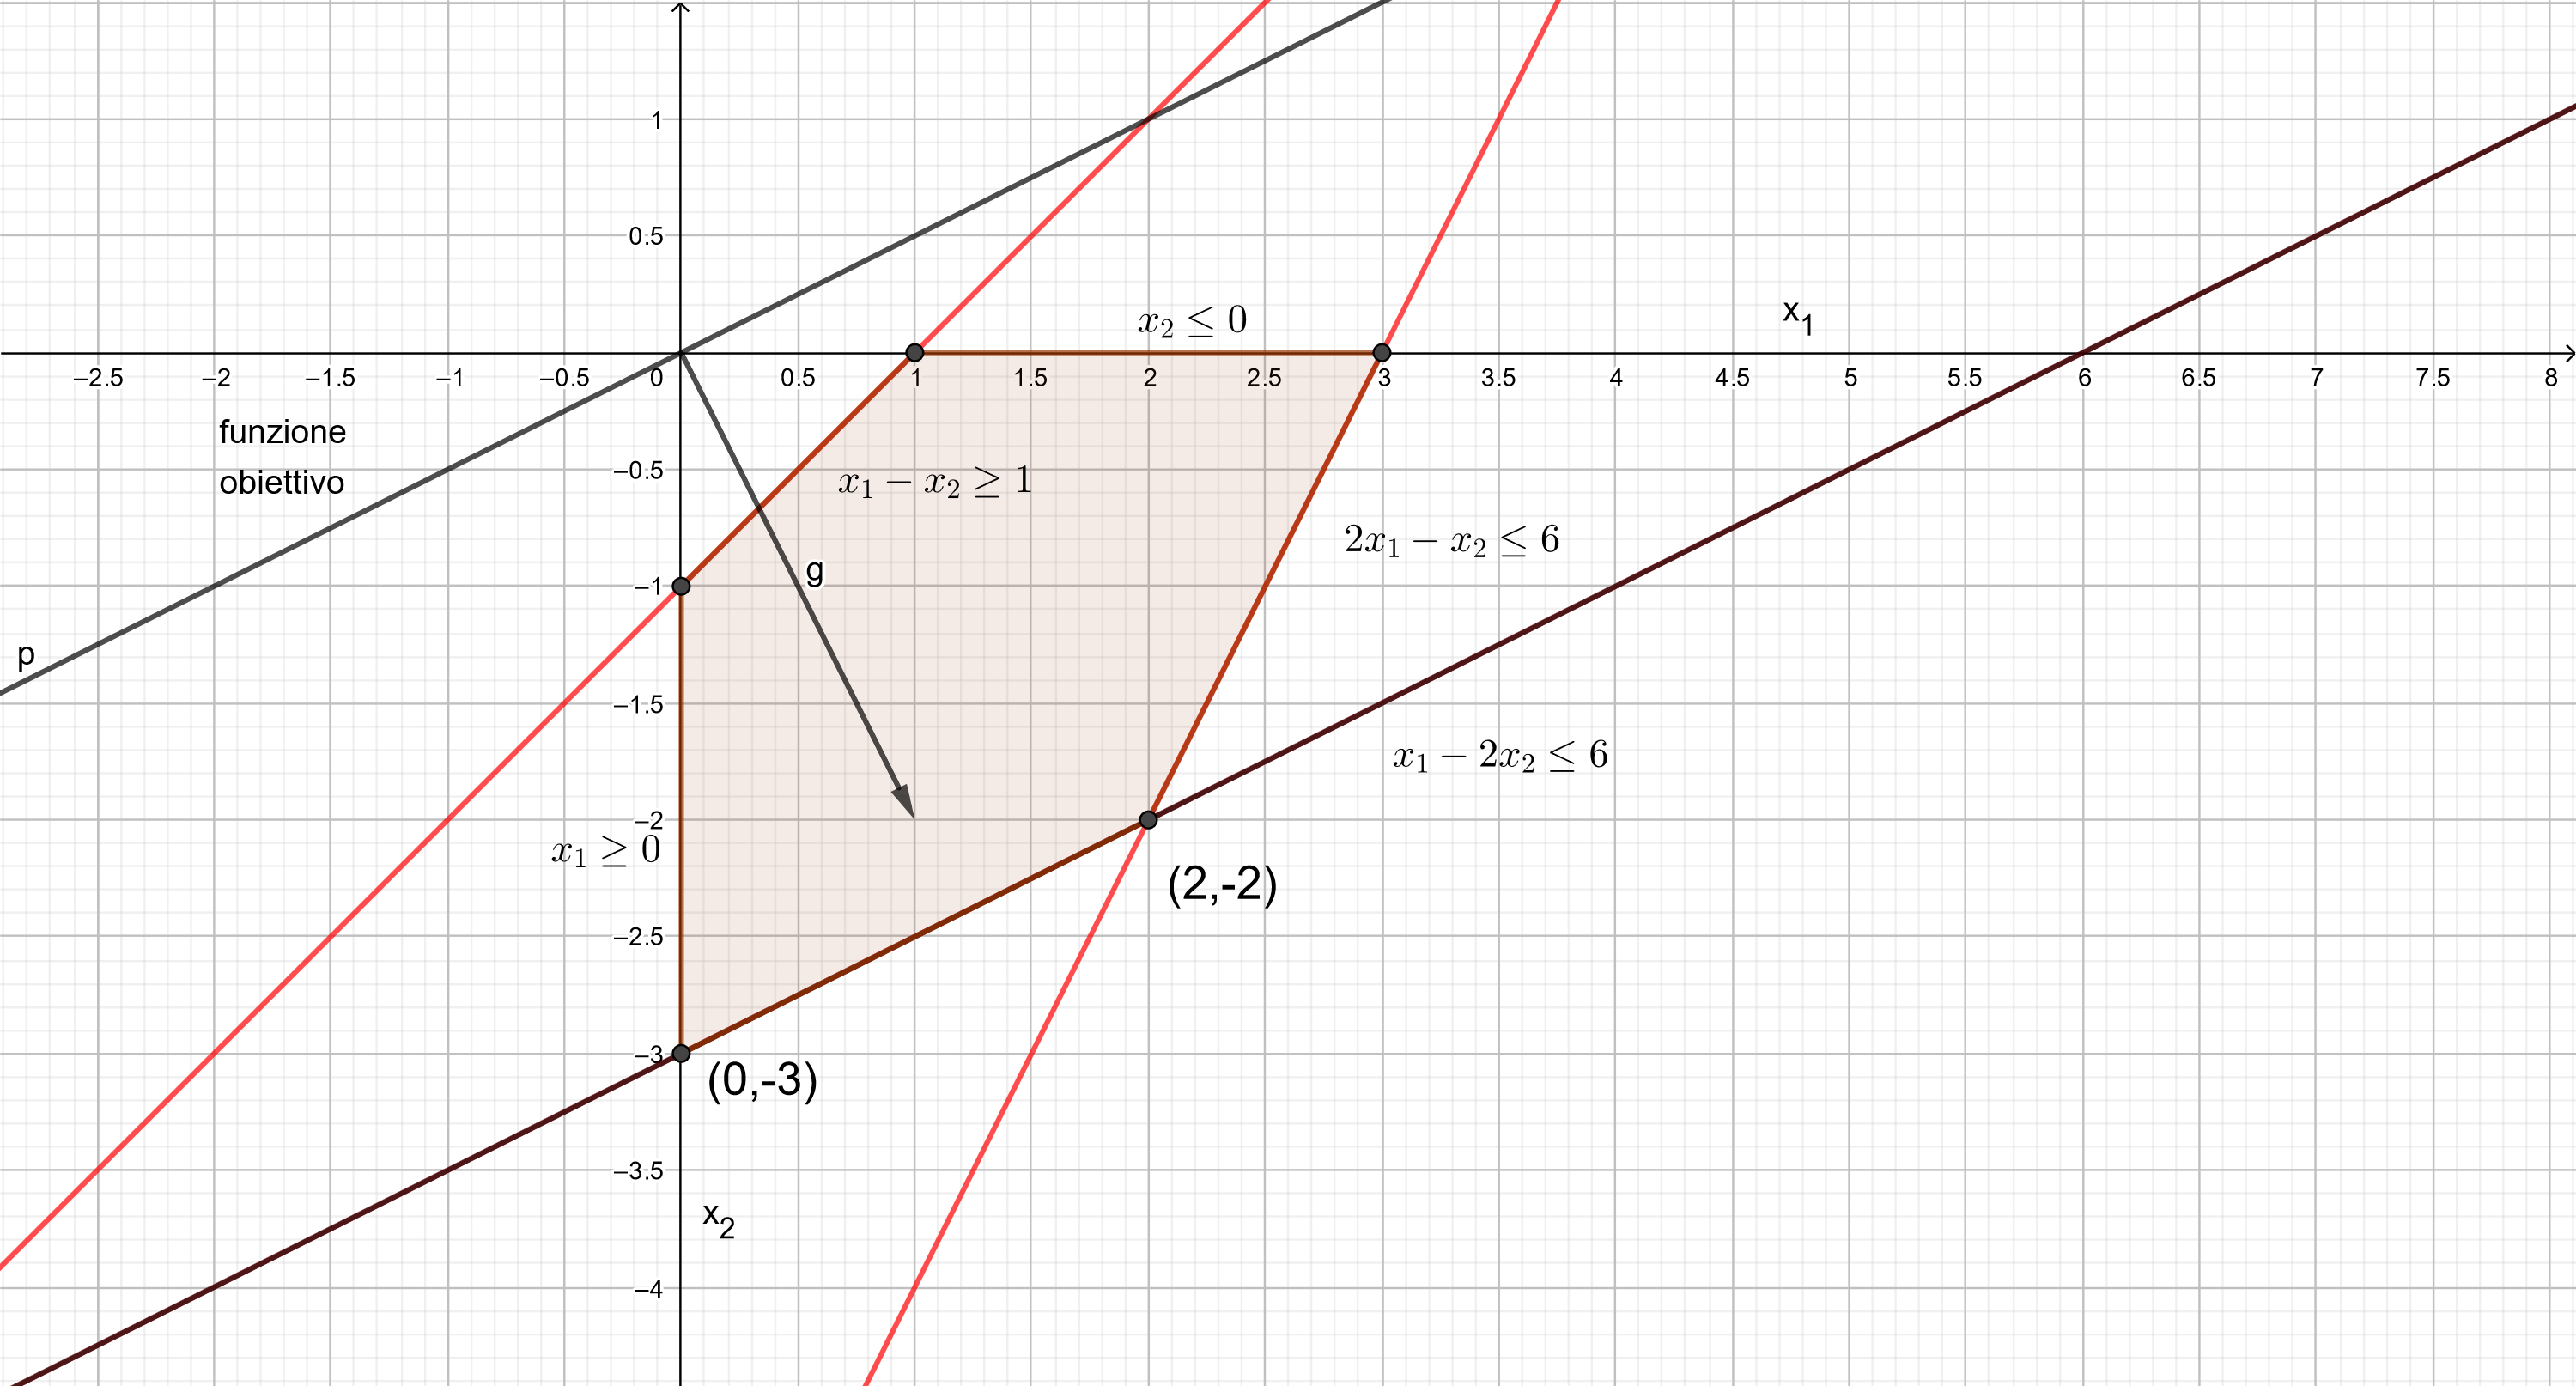
\includegraphics[width=12cm]{seconda-fase.png}
    \end{center}

    Il vettore del gradiente della funzione obiettivo $g$ = <$1, -2$> , composto dalle derivate parziali delle componenti della funzione obiettivo, e' perpedincolare al vincolo $x_1 - 2x_2 \leq 6$.
    Il problema ha \textbf{Infinite Soluzioni Ottime}.
    Le soluzioni sono tutte le coppie <$x_1, x_2$> che risiedono nello spigolo della regione obiettivo su cui si poggia il vincolo $x_1 - 2x_2 \leq 6$.
    Per calcolare il segmento e' sufficiente calcolare l'intersezione del vincolo $x_1 - 2x_2 \leq 6$ con i vincoli $2x_1 - x_2 \leq 6$ e $x_1 \geq 0$.
    Il risultato sono i punti: ($2, -2$),  ($0, -3$). Le soluzioni sono tutti i punti compresi nel segmento delimitato da essi.

    \section{Costriuire il problema duale}
    
    TODO
    
    \section{Calcolare la soluzione ottima del duale utilizzando la teoria della dualita'.}
    
    TODO

\end{document}